\section{Memory Usage Model in Tasks}

%// 模型的作用是什么没有说

%// 1,这些丰富的function API的特征是什么
%// 2,分类的原因
%// 3,通过实验证明有这四类的分类

%Some tasks use less memory to complete the work, while others cost much memory space as they produce massive long lived data objects. One of the major reasons is the function APIs in the processing pipeline. Although different frameworks provide different function APIs, they all have similar characteristics when measuring memory usage. We build models to describe the memory usage characteristics of a function API, and use memory usage rate to determine which model the task belongs to.

As discussed in previous section, some tasks consume less memory while some use much more memory as they produce massive long living data object, which are mainly generated by function APIs in the processing pipeline. Although there are various function APIs, some of them manifest a similar characteristic in terms of memory usage. Based on this observation, we build the models to capture the memory usage characteristic of a function API, and then the memory usage rate is used to determine which model the task belongs to.

%We find that we can build models to describe the memory usage characteristics of a task. Tasks in some models can produce less memory pressure than others because they use less memory to complete the work. One of the major reason is the function APIs in the processing pipeline. Although different frameworks provide different function APIs, they all have similar characteristics when measuring memory usage. We can use memory usage rate to determine to which model the function APIs belong.

\subsection{Memory usage models of APIs}

\begin{table*}[!t]
\small
\centering
\caption{Function APIs in Distributed Data Processing System} 
\begin{tabular}{ c | c | c | c | c | c | c }

\hline
\multirow{2}{*}{\textbf{Community}} & \multicolumn{2}{|c|}{ \multirow{2}{*}{\textbf{Core API} }} & \multirow{2}{*}{\textbf{Application Systems}} & \multicolumn{3}{|c}{\textbf{Partial Function APIs}} \\
\cline{5-7}
 & \multicolumn{2}{|c|}{} & & constant & sub-linear & linear \\
\hline
Hadoop & MapRedcue~\cite{vavilapalli2013apache} & Crunch & Pig, Hive, Yarn & map & reduce & \\
\hline
Microsoft & Drayd~\cite{isard2007dryad} & DryadLINQ & Scope, MadLINQ & map & reduce & join \\
\hline
Spark & \multicolumn{2}{|c|}{RDD~\cite{zaharia2012resilient}} & Spark SQL~\cite{armbrust2015spark}, GraphX~\cite{xin2013graphx} & map & reduceByKey & groupByKey \\
\hline
Flink & \multicolumn{2}{|c|}{Dataset~\cite{www:flink}} & Table~\cite{www:flink}, Gelly~\cite{www:gelly} & where & distinct & join \\
\hline
Google & MapReduce & FlumeJava~\cite{flumejava} & Tenzing, Pregel, Sibyl & parallelDo & combinValue & groupByKey \\
\hline

\hline
\end{tabular}
%\vspace{-2mm}
%\vspace{-4mm}
\label{table:apps}
\end{table*}

A data processing system provides several function APIs, which can be used to implement various applications. These function APIs take as input the input dataset and produce another dataset. The type of data in the dataset may be different. Table~\ref{table:apps} lists the function APIs provided by popular data processing systems. Most function APIs are sourced from MapReduce, a famous computing framework. Other function APIs are used to control the execution of jobs, the typical case of which is the shuffle operations. The shuffle operations are used between the \textit{Map} and the \textit{Reduce} phase, and are regarded as the separation point of a job, because the tasks after the shuffle operations (i.e., \textit{Reduce} tasks) need all results calculated by the tasks before the shuffle operations (\textit{Map} tasks).

These function APIs are all based on key-value pairs: (\textit{K}, \textit{V}). Some function APIs omit the parameter \textit{K} or \textit{V} for the convenience of users. Rather, the default value of the omitted parameters are used during the processes of \textit{map} or \textit{reduce}. The memory space is used by a function API to store the living data objects, because temporary data objects will be reclaimed by the garbage collection. The memory demand determines the characteristic of memory usage. Based on the key-value pairs, the memory size of living data objects is related to both \textit{K} and \textit{V} in the following ways.

\begin{itemize}

\item If the function API does not distinguish the parameter \textit{K}, it processes a record without involving other records. A record will produce a new record accordingly. If the new record is cached in memory, the consumed memory size will certainly increase. If the new record is processed as the input of the next function API or write-to-disk, it will be regarded as a temporary data object and quickly transmitted to the next function API. The size of temporary data object is ignored as it will be reclaimed in the next round of garbage collection.

\item If the function API distinguishes \textit{K}, it will involve all records to process these records with a particular \textit{K}. The function APIs that involve all records are usually called shuffle. While the shuffling stage processes the records to get all \textit{V} with a particular \textit{K}, two operations can be performed on \textit{V}: aggregation and non-aggregation.

\item If the function API does not aggregate the \textit{V}, it only puts \textit{V} in a collection without involving other \textit{V}. The collection contains the intermediate data and has a long lifetime because it is alive until the task processes all records. The collection is usually called the shuffle buffer. After a record is processed, the size of the collection increases by one element and thus the memory size of the shuffle buffer must increase.

\item If the function API aggregates the \textit{V}, the intermediate collection will be replaced by the aggregated value. We also call these data objects with long lifetime the shuffle buffer. Aggregation of \textit{V} means some operations will be performed on all \textit{V} with a particular \textit{K} and produce a new value. Thus, the resulting memory size of the collection will increase when \textit{K} has not appeared yet.

\end{itemize}

As the operations on \textit{K} and \textit{V} decide the size of the living data objects in memory, we build four models in this work to measure the memory usage of each function API when it processes a unit of data. The models are based on the size of the records that are processed, not on the number of the processed records, because the size of a record in each dataset is different. Memory usage refers to the memory space used to store the data objects with long lifetime except the garbage data objects. The four models are shown in Figure~\ref{fig:mur}. We determine the memory usage model of a function API by using the following lemmas.

\begin{figure}[!t]
\centering
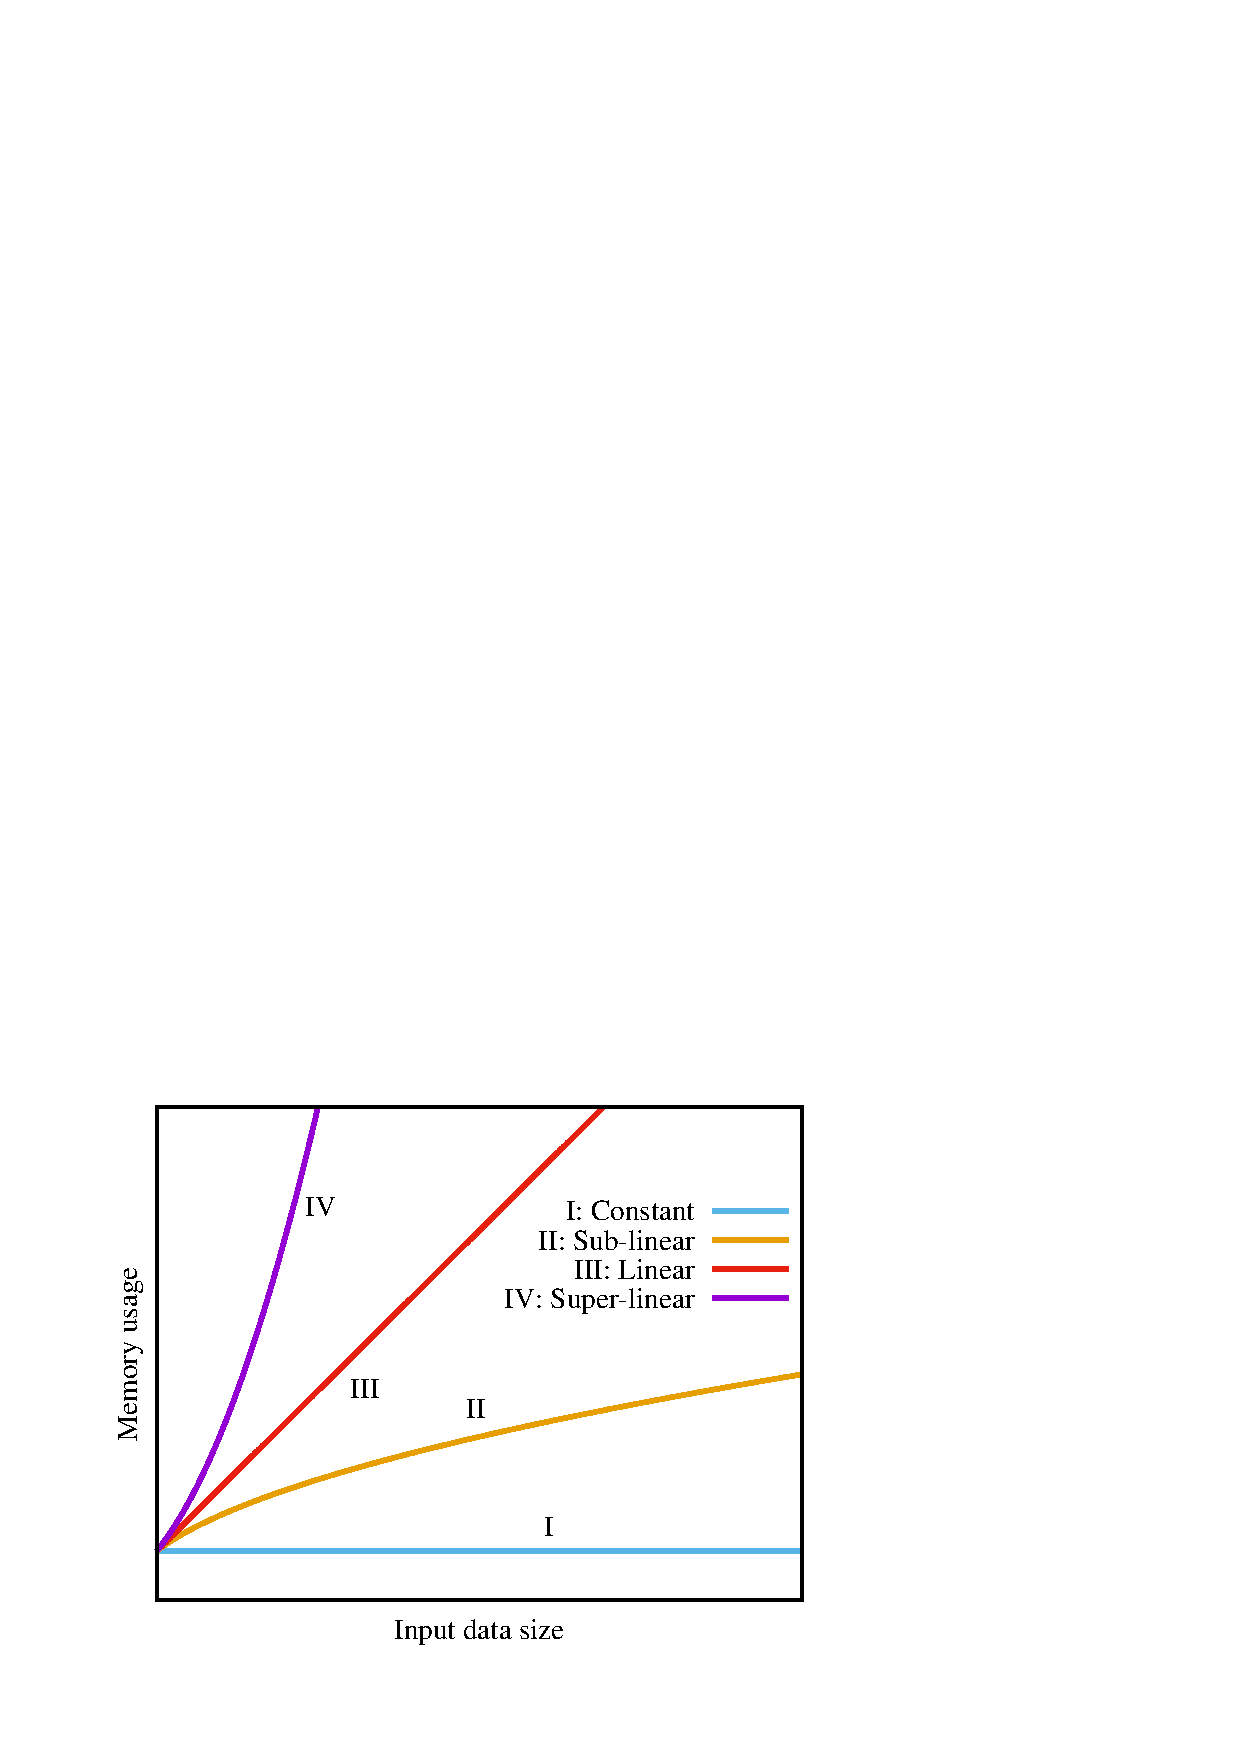
\includegraphics[width=0.3\textwidth]{mur.pdf}
%\vspace{-2mm}
\caption{Four coarse-grained models of function API}
%\vspace{-4mm}
\label{fig:mur}
\end{figure}

\newtheorem{lemma}{Lemma}
\begin{lemma}[Constant] The memory usage model can be defined as constant (Line I in Figure~\ref{fig:mur}) only when the following conditions are true:
\begin{enumerate}
\item The function API does not distinguish the key, \textit{K};
\item The resulting data will not be cached in memory.
\end{enumerate}
\end{lemma}

\begin{lemma}[Sub-Linear] The memory usage model can be defined as sub-linear (Line II in Figure~\ref{fig:mur}) only when the following conditions are true:
\begin{enumerate}
\item The function API distinguishes the key, \textit{K};
\item The function API aggregates the value, \textit{V};
\item \textit{K} appears randomly in the input dataset.
\end{enumerate}
\end{lemma}

Note that the reason why we require that \textit{K} appears randomly is because the size of intermediate data will increase only when the \textit{K} has appeared. If most \textit{K} gathers around some neighbouring records, the size of intermediate data will increase linearly.

\begin{lemma}[Linear] The memory usage model can be defined as linear (Line III in Figure~\ref{fig:mur}) when the following conditions hold:
\begin{enumerate}
\item The function API distinguishes \textit{K};
\item The function API does not aggregate \textit{V}.
\end{enumerate}
\end{lemma}

Both cache operations and the appearance pattern of \textit{K} affect the  size of intermediate data. Thus although some function APIs have the same operations on \textit{K} and \textit{V}, their memory usage models may be different. The constant model requires that intermediate data are not cached in memory. The increasing model is determined by the size of the cached data objects. The sub-linear model also requires the random appearance of \textit{K}. When a function API does not satisfy the above conditions, we need to redefine their models. In other words, the model is defined not only by the function APIs, but also by the user-defined function or data distribution. The memory usage model should be redefined when the following conditions are true:

\begin{itemize}

\item If the function API does not distinguish the \textit{K} and the result data are cached in memory, the speed of increasing size in memory can be 1) \textit{linear} (Line III in Figure~\ref{fig:mur}) when the function API does not work based on formal result; 2) \textit{super-linear} (Line IV in Figure~\ref{fig:mur}) when the function API produces larger result data, such as computing a histogram of the appeared numbers and all their divisors; 3) \textit{sub-linear} (Line II in Figure~\ref{fig:mur}) when the function API produces smaller result data along with the computation. 

\item If a function API i) distinguishes \textit{K}, ii) does not aggregate \textit{V}, iii) \textit{K} has not appeared yet in the input dataset or the appearance of \textit{K} is not random. The memory usage model of the function API should be linear.

\end{itemize}

Note that when function APIs belong to the same linear model, they can also be distinguished because the slope of the line in Figure~\ref{fig:mur} may be different. Steeper the slope is, the heavier impact the API function has on memory pressure. Based on the slope and four models, we can distinguish all function APIs in various data processing systems.

%If one function API does not satisfy one of the lemmas, we define them as the super-linear model. One possible super-linear model is shown as the Line IV in the figure. However, we find that no function API can be defined as the super-linear within the range of our research, most function APIs will show the memory usage as other three models in our evaluations.

%We should notice that the caching data and shuffle buffers are both long lifetime data objects in memory. Shuffle buffers are lived along with the shuffle operation. Some systems provide combine in map side which will effect the shuffle operation. When tasks need combine in map side, the function API will be executed in both map tasks (write) and reduce tasks (read). But when it needs not to combine, the function API will only be executed in reduce tasks, the map tasks will just produce the K-V pairs without any process. Other temporary data objects in function APIs will be reclaimed by garbage collection immediately.

%Some function APIs need both ensured \textit{K} and \textit{V}, such as \textit{shuffle}. According to the operations implemented on the \textit{V} with the same \textit{K}, these shuffle function APIs can be split to two groups: aggregate and non-aggregate. Aggregate operations are used to aggregate \textit{V} with the same \textit{K}. In this case, whether the result data in memory should increase the size is decided by the \textit{K}. But it's sure that non-aggregate operations must increase the size of result data in memory because no matter whether the \textit{K} has repeated emergence, \textit{V} is appended to the result data. What's more, besides the operations themselves affect the memory pressure, the type of \textit{V} also make some impact on the memory pressure. While the operations in running tasks are the same, we can also distinguish the influence on memory pressure by the data class they process.

%Some frameworks directly provide the \textit{cache} function API to cache the data in memory. This operation is different to other operations because it just applies for a memory space to store the dataset. JVM heap is usually the default region to store these data. Forward frameworks also provide storing off heap to save the execution memory space. No matter where the dataset store in, we just regard these memory pressure from JVM heap or system memory as unify.

%Most function APIs can satisfy these three items. Other function APIs, such as \textit{cache}, are designed to lengthen the lifetime of intermediate data but not influence the memory usage during processing. Further function APIs are also used to control the execution of jobs, the typical case is shuffle operations. Shuffle operations are used between Map and Reduce, and regarded as the break point of jobs. Because tasks after shuffle operations (reduce tasks) need all results of tasks before shuffle operations (Map tasks).  

\subsection{Memory usage models in tasks}
\label{subsec:taskmodel}

A task is implemented by at least one function API. Some systems define only one function API in each task, such as Hadoop. Other systems define the function APIs in a task according to the shuffle operations in the user-defined program, such as Spark and Dryad. As the shuffle operations are used to split the jobs, they implement both shuffle write and shuffle read. Thus, we consider the memory usage of a task in three phases: read, process, and write. The read and write phase of a task only contain one shuffle function API, or no function API if they read/write from/to disk or print in screen. If a task has a process phase, the phase contains several function APIs. 

The read and write phases of a task have independent memory usage models with a strict order. However, the memory usage model of the process phase is different. A function API in the process phase is always of the constant model. They never distinguish  \textit{K} and do not need to calculate all intermediate data. Thus they process each record as a temporary data object and quickly pass the intermediate data to the next function API. All constant models will not be shown in the memory usage of a task if the write phase of the task has the shuffle operations. This is because the size of the shuffle buffer is much bigger than the constant models. However, when the task caches intermediate data in memory, these intermediate data will be transmitted to the next function API after completing the current function API. Under this circumstance, the model is redefined. The redefined model will be combined with the independent models in a task. When there are several memory usage models in a task, we can only monitor the current memory usage model when we schedule the task. When reducing the current memory pressure, we use the current memory usage model to calculate the memory usage of the task.

Based on the memory usage models in a task, we only need the slope of each line in Figure~\ref{fig:mur} to determine the current memory usage model. We term the slope the \textit{memory usage rate}. Thus, the memory usage rate of a task is defined as the memory size of the newly produced long-living data objects when a task processes a unit of input data.

%It is clear that when the function API distinguishes the \textit{K} and not aggregates the \textit{V}, the memory usage of result data will increase after each record is processed. Thus it will have stable necessary of memory space compared to sub-linear model. The linear model can be defined as the Line III in Figure~\ref{fig:mur}. We notice that as the slope of line can be different, linear model can also have different impact on the memory pressure. The slope can be decided by the type of result data.

%Some special tasks will be redefined as linear too. The first one is when tasks cache data in memory. When the result data of constant model is cached in memory, the memory usage will increase undisputed. However, it is not applicative for sub-linear type because the result data has already stay in memory with long lifetime. The second one is the appearance of \textit{K} when some function APIs distinguish \textit{K}. When the appearance of \textit{K} is not balanced, the memory usage will also increase after processing one record. Thus these function APIs will also be redefined as linear.

%Function APIs are transparent to tasks and running discrepant with different dataset, and it's not sensible to clearly distinguish which function API the task executes. Although, we can coarse-grained distinguish these function APIs along with the input dataset features. Memory usage rate of a task combines the features of both function API and input dataset: i) different operations result in different growth pattern of middle data in memory, which means the influence on memory pressure; ii) the data class of input dataset decides the size of each record (key-value pairs as usual) in memory. 


%If function APIs in one task cannot satisfy any of the lemmas, we define them as the super-linear. One possible memory usage model of super-linear is shown as Line IV in Figure~\ref{fig:mur}. super-linear type is rare in current data processing systems. Anyhow we build this model to cover these complex function APIs.

%\textbf{Constant} Simple function APIs that come from \textit{map} are both constant model, such as \textit{map}, \textit{flatMap}. These function APIs process one record and result in another record. Thus the result data in memory is ensure. We should notice that most result data processed by these function APIs will not be stored directly in the memory, they have three different directions: i) used in next function API. The function APIs with constant model in this scene just produce the middle result for next function, thus these data in memory are all temporary variables which just occupy a constant space. ii) saved to disk. The data produced will be directly write to file stream, thus a constant memory space are occupied also. iii) saved to memory. This scene does not accord with the constant type, because each result data is saved in memory and the occupied space are linearly growth.  

%\textbf{Sub-linear} Most aggregate function APIs can be sub-linear, such as \textit{reduceByKey} and \textit{reduce}. The root of sub-linear is the repeatability of \textit{K}. When the aggregate function APIs aggregate \textit{V}, if \textit{K} has existed the result \textit{V} will just be update, thus the occupied space remain unchanged; if \textit{K} is new and a new record will be append to the result data, the occupied space will increase. However, this coarse-grained model is based on the equally distributed \textit{K}. We can just weak this type to linear type if the layout of K not satisfies this rule, although this type has less memory usage than linear type.

%\textbf{Linear} Non-aggregate function APIs are the most directly type because it's clear that when processing one record the result data in memory must increase its size, such as \textit{groupByKey} and \textit{join}. No matter whether \textit{K} has existed, \textit{V} will be append to the data object with the same \textit{K} in result data. Although  most tasks with non-aggregate function APIs or weak sub-linear type are regarded as linear type, we can still distinguish these tasks by the slope. The slope of the linear are decided by the result data class. Complex data class will occupy more memory space than simple data class, which means the slope of the linear in memory usage are larger. The larger slope in memory usage rate is considered to lead to more memory pressure compared to tasks with low slope in memory usage rate.

%\textbf{Super-linear} Super-linear type is rare in current data processing systems. A typical function API is \textit{flatMap} which flats the record (the data class of record should be collection) to records one by one. Although flatMap provides the flatten operation, if the map operation inside doesn't extend the size of each record, the memory usage rate type of this task is also linear or constant. Anyhow we build this type to cover these complex function APIs with super linear memory usage rate. 

%After the coarse-grained type of all running tasks are ensured, we can coarsely distinguish which task can lead to more memory pressure when we consider the memory usage rate. Based on the coarse-grained model, we can apply for memory usage rate based scheduler to mitigate the memory pressure.

